\chapter{Dostupné testovací nástroje}
V kapitole dostupné testovací nástroje bude zkoumána část dostupných opensource i komerčních nástrojů pro všechny fáze testování. U všech testovacích nástrojů bude posuzován přínos v případě nasazení v testovacím systému pro výrobky společnosti Conel.

\section{Jenkins CI}
Jenkins CI je nástroj pro kontinuální integraci. Kontinuální integrace spočívá v častém kompilování zdrojového kódu a následném spouštění testů nad tímto softwarem.
Jenkins je nástroj napsaný v programovacím jazyce Java. Tento nástroj má podoru kompilace různých projektů díky veliké možnosti nastavení a díky velké podpoře pluginů, jejichž počet neustále roste.

\begin{figure}[h]
  \centering
  
\includegraphics[width=.3\LW]{jenkins_logo}
  \caption{Logo produktu http://www.jenkins-ci.org}
  \label{fig:testlink_logo}
\end{figure}

Jenkinsen je dobrý a přehledný buildovací systém s podporou mnoha programovacích jazyků. Velikou výhodou tohoto systému je opensource řešení projektu. Naopak nevýhodou jsou veliké systémové požadavky nástroje. Tento systém sice podporuje testování, ale podporuje pouze testování na úrovní testování jednotek, které v navrhovaném systému nebude vůbec použito. Naopak nepodporuje funkční a systémové testování na konkrétním hardwaru, které bude v testovacím systému využíváno.

\begin{figure}[h]
  \centering
  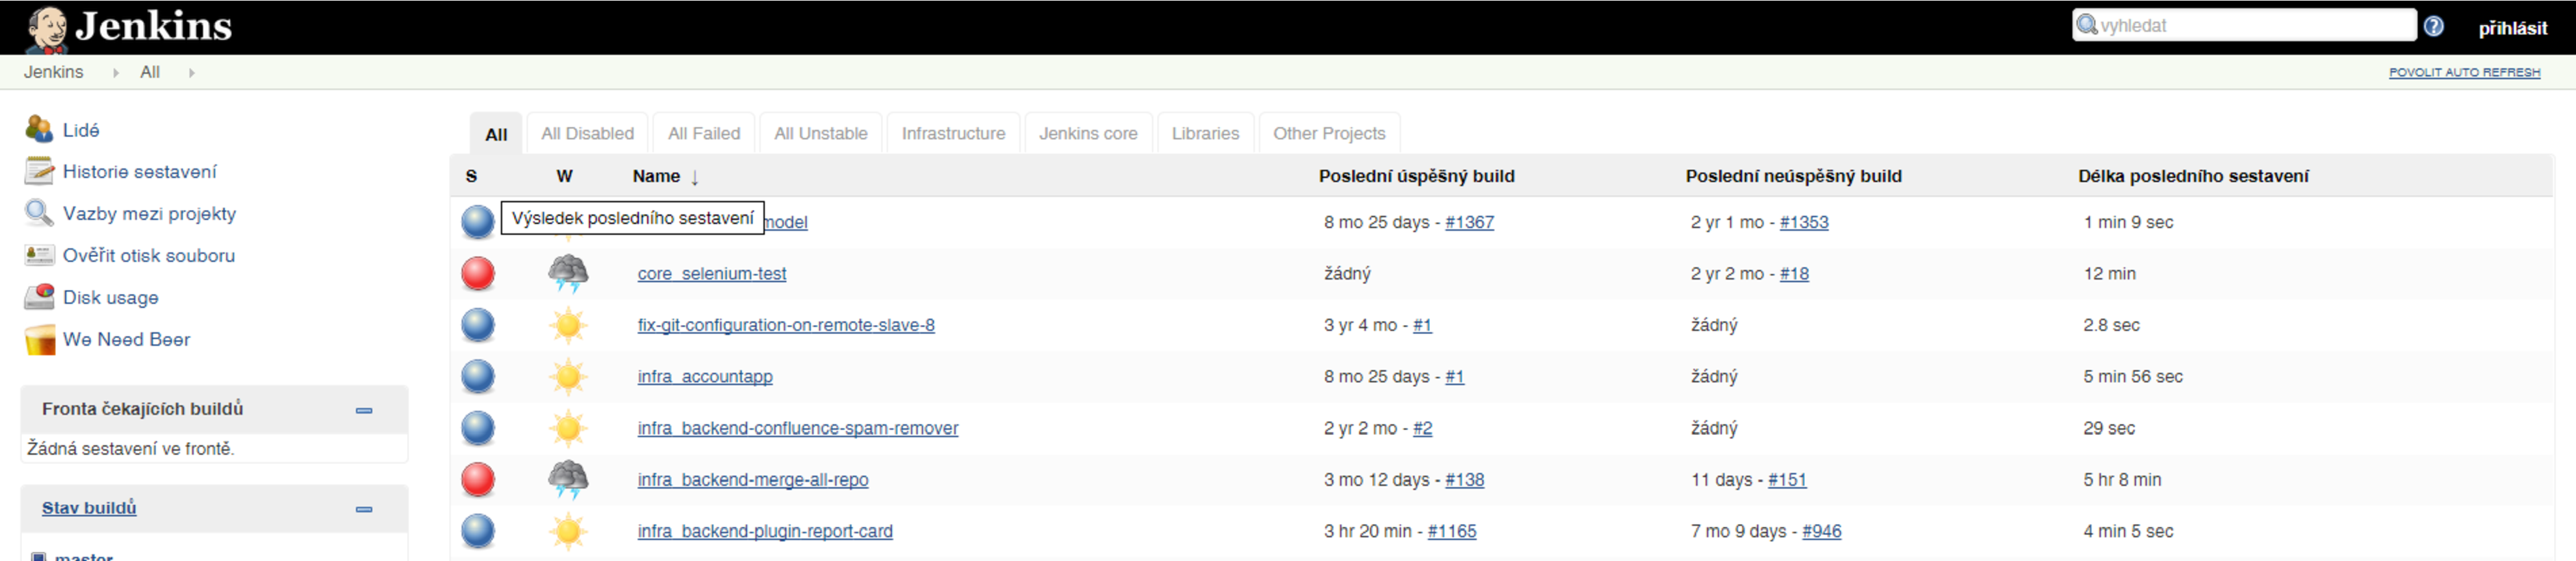
\includegraphics[width=\LW]{jenkins_example}
  \caption{Příklad otevřené aplikace Jenkinsen}
  \label{fig:testlink_example}
\end{figure}

Použití tohoto nástroje pro konitunální integraci v testovacím zařízení by bylo možné pouze ve fázi buildování všech firmwarů. Skripty zajišťující správnou funkci s buildovacím program ltib je potřeba napsat stejné jak při použití systému Jenkins, tak při vlastním spouštění překladu. LTIB je image systém používající se pro překlad většiny výrobků. Taktéž samotné spouštění těchto skriptů bude v testovacím systému již implementováno v části obsluhující spouštění testovacích skriptů. Na zákldě těchto skutečností jsem upřednostnil použití vlastního spouštění kompilačních skriptů, hlavně z důvodu jednotného systému pro vizualizaci všech informací o průběhu všech fází překladu a testování.

\section{Testlink}
Testlink je nástroj pro správu a organizaci testů. Nástroj je dělaný jako webová aplikace napsaná v jazyce PHP využívající databázi MySQL nebo PostgeSQL. Aplikace je zdarama i pro komerční účely, jelikož je šiřená pod licencí GPL.

\begin{figure}[h]
  \centering
  
\includegraphics[width=.3\LW]{testlink_logo}
  \caption{Logo produktu http://www.testlink.org}
  \label{fig:testlink_logo}
\end{figure}

Nástroj testlink umí dobře spravovat a organizovat testy a testovací případy. Nástroj obsahuje pět základních pilířů o které se dále opírá a tvoří jeho strukturu. Prvním a základním prvkem je testovací případ neboli test case. Tato položka odpovídá již odpovídajícímu testovacímu skriptu či testovací proceduře popisované ve způsobech testování. Dalším prvkem je sada testů označovaná test suite. Sada testů organizuje testy do funkčních skupin. Třetím prvkem nástroje testlink je testovací plán. Testovací plán je sestaven ze sad testů a dále z informací o daném testování. Dalším prvkem je testovací projekt, který je základním prvkem systému. Testovací projekt v známé terminologii odpovýdá testovanému subjektu. Posledním prvkem tohoto systému je uživatel. Jednotlivý uživatelé maji různá práva úprav v systému, aby byla zavedena bezpečnost systému. Tento systém umí dále podle vložených výsledků testů vytvářet reporty o testování v různých formátech.

\begin{figure}[h]
  \centering
  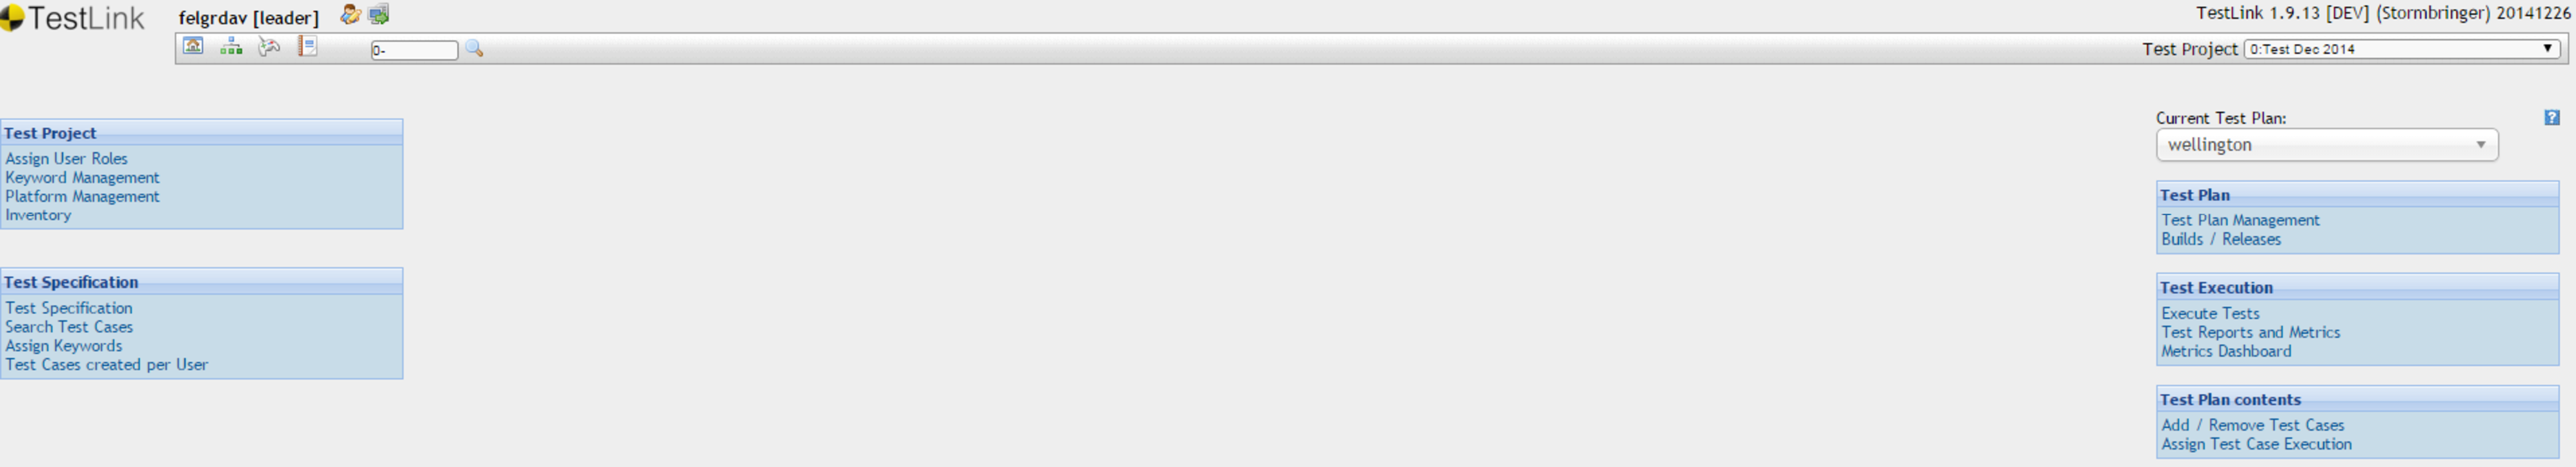
\includegraphics[width=\LW]{testlink_example}
  \caption{Příklad otevřené aplikace Testlink}
  \label{fig:testlink_example}
\end{figure}

Nástroj Testlink může být účiný v případě manuálního testování pro snadnou správu testů a reportování výsledků těchto testů. I v případě testovacího systému společnosti Conel by bylo možné systém nasadit. Pokud by byl systém nasazen byly nutné úpravy tohoto systém k požadavkům automatického testování a speciálním požadavkům na modulárnost testovaných výrobků. Po krátkém zkoumání jsem zjistil že úpravy pro automatické testování a úpravy k potřebám hiearchie testovací laboratoře by byli rozsáhlé. Dále tento systém působí velmi nepřehledně. Díky těmto závěrům bylo rozhodnuto nepoužití tohoto nástroje pro spravování testů a reportování výsledků.

\section{Selenium}
Selenium je nástroj pro testování webových aplikací. Tento nástroj je také opensource program napsaný v jazyce Java. Selenium je dostupné ve čtyřech variantách a to Selenium IDE, Selenium RC, Selenium WebDriver a Selenium Grid. Selenium IDE je plugin do internetového prohlížeče Firefox. Dále Selenium RC, který si sám pouští internetové prohlížeče a provádí na nich testy. Testy je možné psát v jazycích Java, C, Python, Ruby, Perl, PHP a je pro psaní těchto testů připraveno přehledné API. Seleneium WebDriver usnadňuje psaní samotných testů na úkor nutnosti psaní všech testů na každý prohlížeč. Poslední Selenium Grid umožňuje paralérní spouštění testů na více strojch i počítačích.

\begin{figure}[h]
  \centering
  
\includegraphics[width=.1\LW]{selenium_logo}
  \caption{Logo produktu http://www.seleniumhq.org}
  \label{fig:selenium_logo}
\end{figure}

Selenium je dobrý nástroj pro testování webových aplikací. Nástroj bude určitě využitelný i pro testování samotných routerů. Bohužel v první fázi budou jednotlivé konfigurace měněni pomocí ssh a telnet přístupu do routeru. Jelikož tento nástroj více možností neobsahuje, tak nebude v první fázi nasazování testovacího zařízení použit.

\section{VectorCAST}
Nejlepším zkoumaným testovacím nástrojem byl komerční produkt VectorCAST od společnosti VECTOR Software. VectorCAST je platforma přímo určená k testování embedded zařízení podporující velkou škálu zařízení a testů.

\begin{figure}[h]
  \centering
  
\includegraphics[width=.4\LW]{vector_logo}
  \caption{Logo produktu http://www.vectorcast.com/}
  \label{fig:vector_logo}
\end{figure}

Samotný produkt je rozdělen do několika částí které jsou dodávány zvlášť podle potřeb zákazníku a typu cílové testované aplikace. První dva programy se zabývají testováním jednotek a integračním testováním. První program je VevtorCAST/Ada, který je určen pro testování softwaru napsaném v jazyce Ada. Ada je robustní staticky typovaný programovací jazyk, který je určen pro programování krityckých aplikací. Tento jazyk v testovaných zařízeních nikdy nebyl použit a tak se dále tímto programem nebudu zabývat. Druhým programem určeným pro testování jednotek a integrační testování je VectorCAST/C++ určeným pro aplikace psané v jazycích C a C++.

VectorCAST/C++ je řešení pro automatizované testování jednotek a integrační testování. Tento nástroj přímo automatizuje vytváření unit testů pro samotný zdrojový kód. Nástroj je možné spustit nativně nebo na konkrétní cílové platformě. Pro spouštění na cílové platformě je potřeba nástroj VectorCAST/RSP, který bude popsán později. Další vlastností tohoto systému je jednoduché regresní testování softwaru, kdy je možné automaticky spouštět již vytvořené testy. Nástroj může pracovat ve dvou módech a to Source mód a Agile mód. První Source mód tvoří testy z modulů, které jsou již implementovány. Druhý Agile mód nepotřebuje pro tvorbu testů zdrojové kódy daného modulu, ale stačí mu pouze jeho hlavičkové soubory.

\begin{figure}[h]
  \centering
  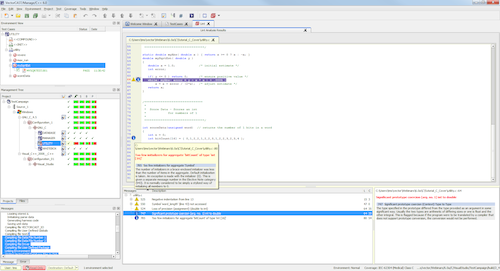
\includegraphics[width=\LW]{vector_example}
  \caption{Příklad otevřené aplikace VectorCast}
  \label{fig:vector_example}
\end{figure}

Pro lepší správu regresního testování slouží nástroj VectorCAST/Manage. Nástroj je vhodný pro vývoj aplikací s dlouhým životním cyklem, či s většímy vývojovímy týmy. Členové celého týmu mohou pohodlně spouštět regresní testy a sledovat jejich výsledky. Nástroj dále obsahuje podporu testování aplikace na více operačních systémech, více cílových platformách a různých konfiguracích. Testování stejného modelového případu ve všech možných situacích je důležité pro stoprocentní otestovanost systému. Nástroj umožňuje také funkci testování založené na změnách, kdy nástroj sleduje změny zdrojový kódů a spouští pouze testy modulů na kterých byli provedeny změny.

VectorCAST/Cover analuje využití kódu v průběhu systémového testování. Pomocí tohoto nástroje je možné zjistit jaká část aplikace nebyla při samotném systémovém testování testována. Druhým nástrojem pro analýzu kódu VectorCAST/MCDC můžem provést analýzu všech možných stavů a podstavů kam se aplikace psaná v jazuk C či C++ může dostat.

Testované aplikace je možné testovat přímo na cílové platformě pomocí již dříve zmíněného nástroj VectorCAST/RSP. V tomto nástroji je implementována široká škála kompilátorů. Pomocí tohoto nástroje lze stáhnout testovací postup přímo na cílovou platformu, kde jsou všechny testy provedeny a výsledky odeslány zpět testovacímu zařízení. Všechny kroky probíhají automaticky na pozadí bez interaktivity obsluhy.

Řešení pro testování embbeded aplikací VectorCAST a jeho všechny doplňující balíky jsou velmi silným nástrojem. Po detailní zkoumáním tohoto nástroje a jeho funkcionalit nemohu ani tento nástroj doporučit pro účely automatické testování výrobků společnosti Conel. Hlavním důvodem nevhodnosti použití tohoto nástroje je potřeba zdrojového kódu k tvorbě jak testování jednotek, tak integračního testování. Firmware v testovaných výrobcích je z devadesáti procent tvořen opensoource projekty. Z toho vyplívá tvorba takových testů na všem software by byla velmi dlouhá práce s nejasným výsledkem. Dále projekt neobsahuje žádnou podporu systémového testování a modulární návrh testů.

\section{Maveryx}
Maveryx je komerční řešení pro automatizované testování aplikací s grafickým uživatelským rozhraním. Tato aplikace podporuje testování aplikacích napsaných v jazyce Java a aplikací pro operační systém Android. Aplikace Maveryx se nebude hodit k použití v testovacímu systému, ani k řešení žádného mezikroku testování.

\section{Robot Framework}
Robot Framework je automatický framework pro akceptační testování a vývoj řízený testy. Základní testovací možnosti lze rozšířit pomocí nových knihoven napsaných v jazyce Java nebo Python, pomocí kterých je možnost doplňovat nová klíčová slova.

\begin{figure}[h]
  \centering
  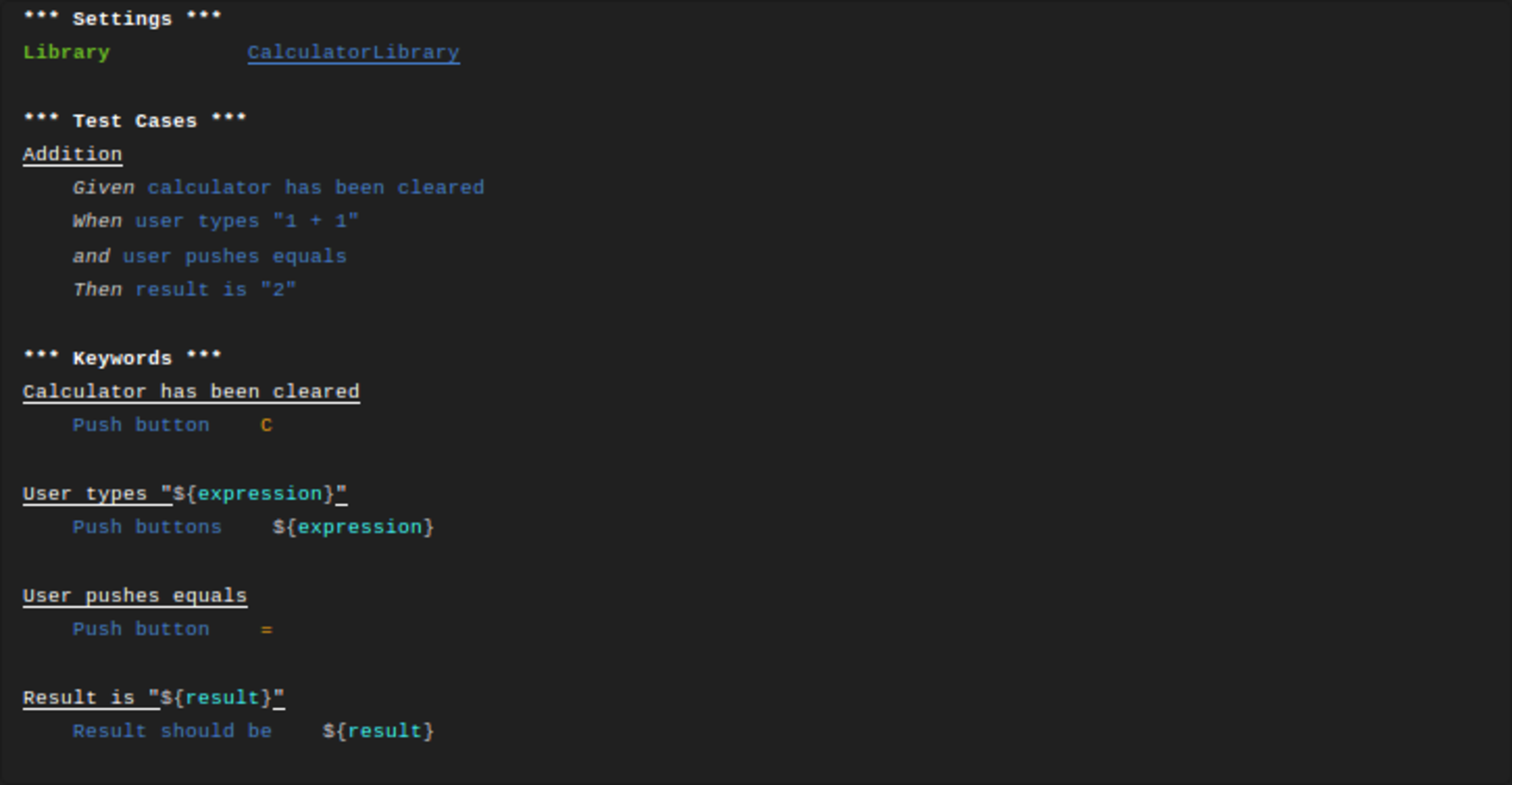
\includegraphics[width=\LW]{robot_example}
  \caption{Příklad testu ve framewotku http://robotframework.org/}
  \label{fig:robot_example}
\end{figure}

Robot Framework je pěkný příklad jak by mohl testovací framework vypadat. Specifické požadavky testovacího frameworku pro testování síťových embedded zařízení tento framework nemá. Samozřejmně by se dali všechny knihovny dopsat pomocí přídavných knihoven a systém upravit k potřebám testovacího zařízení. Jednodušší cestou bude vzít dobré zkušenosti z testování tohoto frameworku a postavit vlastní API vhodné k testovavání embedded aplikací.

Robot Framework je opensource projekt pod Apache Licencí 2.0. Robot Framework je nezávislý na operačním systému a aplikacích, jelkož jádro frameworku používá Python.

\section{Embedded Unit}
Embedded Unit je nástroj pro testování na úrovni testování jednotek. Nástroj je určen pro testování softwaru pro embedded aplikace. Jelikož tuto úroveň testování nebudu prozatím implementovat do testovacího systému, tak nebude tento nástroj prozatím využit.

\section{Linux Test Project}
Linux Test Project má za cíl testování stability, spolehlivosti a robustnosti Linuxového jádra a souvisejících funkcí. Tímto nástrojem bychom mohl testovat Linuxovou distribuci pro danou architekturu procesoru. S takto detailními testy se pro testovací laboratoř prozatím nepočítá, ale pro kvalitní testování výrobků se bude do budoucna hodit.

\section{Ostatní aplikace}
API pro vytváření jednotlivých testů bude využívat různé, převážně opensource programy ze světa síťových technologií. Například Curl pro komunikaci mnoha síťovými protokoli. Všechny tyto použité programy budou popsány v kapitole věnující se API testovacího systému.

\endinput
